
\section{Histogram computation}

A histogram succinctly and meaningfully summarizes the data, thus histogram computation is a very
common analysis task. In this section, we study bit streams that aim to reproduce the most accurate
histogram possible at any bit rate. It is necessary to first define a criteria to compare two
histograms. In the literature, there have been many distance metric proposed for histograms; in the
experiment that follows, we compare eight of the more common distance metrics, namely Bhattacharyya
[CITE], Chi-square [CITE], Earth mover's distance (EMD) [CITE], Total variation [CITE], Hellinger
[CITE], Kolmogorov-Smirnov [CITE], an Kullback-Liebler [CITE]. We use Algorithm [REF] to produce one
stream for each of these metrics and plot their PSNR curves (Figure
\ref{fig:histogram-metrics-comparison}). \ptb{It is not quite clear
  whether these streams are optimized by their correspoinding norm or
  by EMD ?}

\begin{figure}
	\centering
	\subcaptionbox{\emph{boiler}}
	{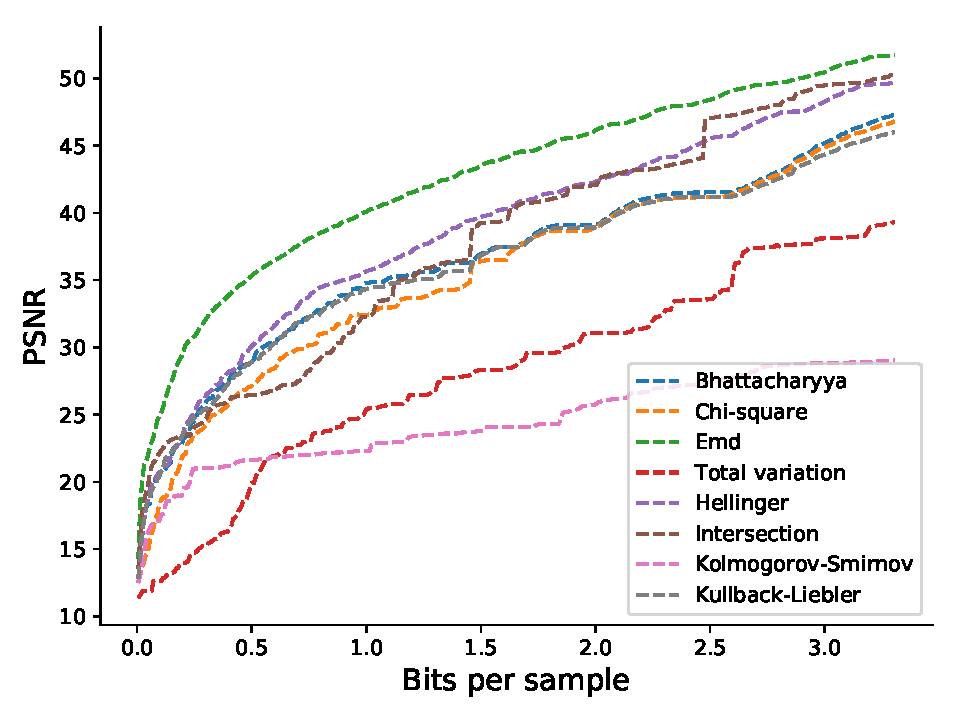
\includegraphics[width=0.48\linewidth]{img/histogram/different-metrics/boiler-histogram-metrics.pdf}}
	\subcaptionbox{\emph{flame}}
	{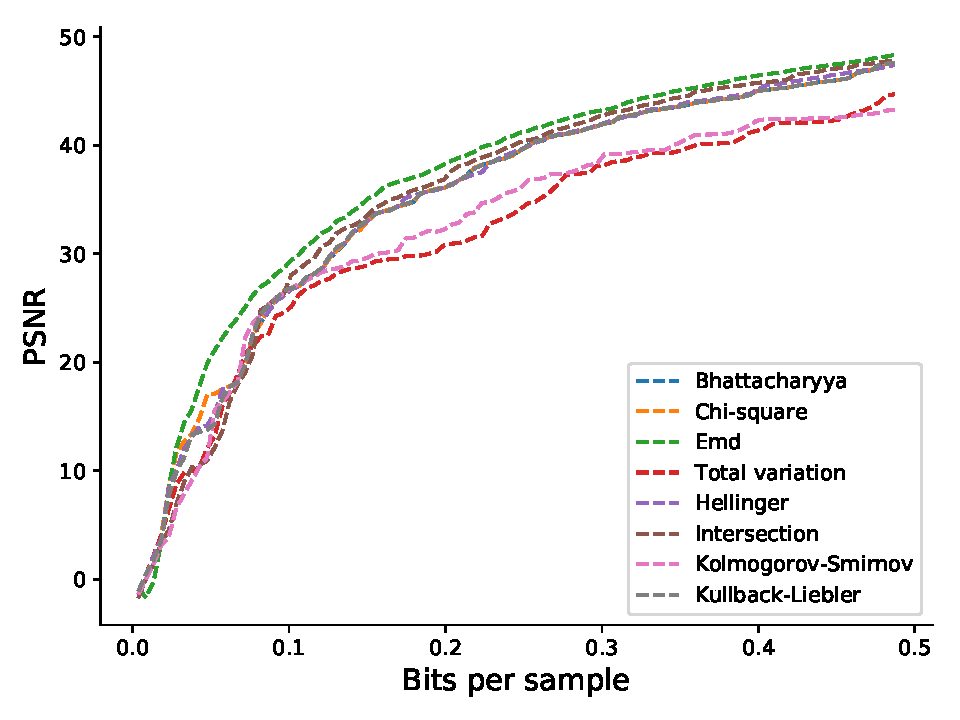
\includegraphics[width=0.48\linewidth]{img/histogram/different-metrics/kflame-histogram-metrics.pdf}}
	\subcaptionbox{\emph{diffusivity}}
	{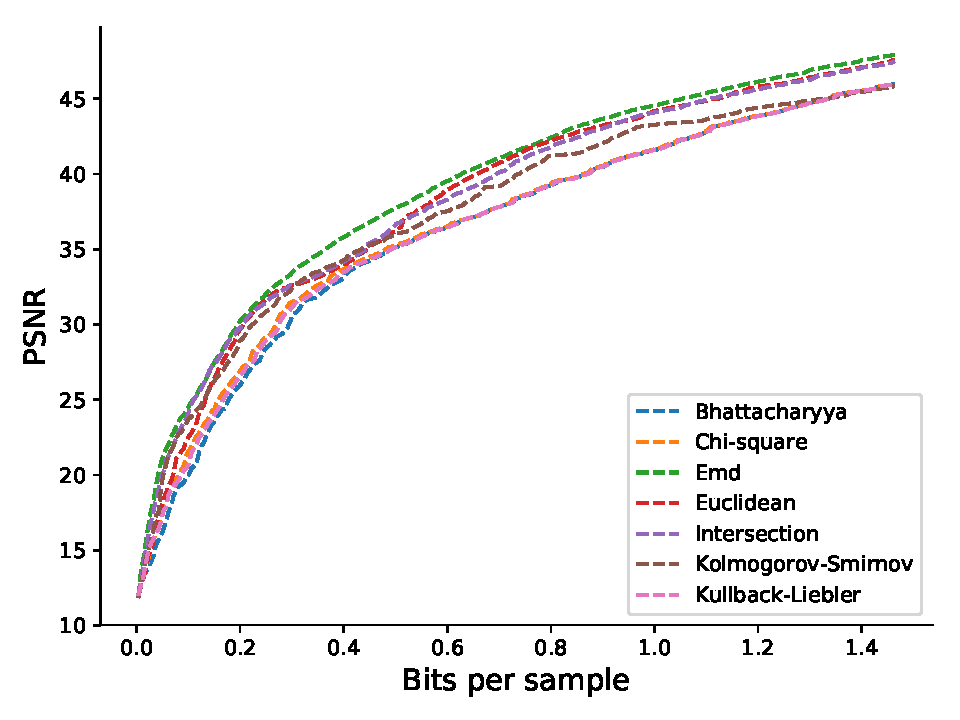
\includegraphics[width=0.48\linewidth]{img/histogram/different-metrics/miranda-diffusivity-histogram-metrics.pdf}}
	\subcaptionbox{\emph{turbulence}}
	{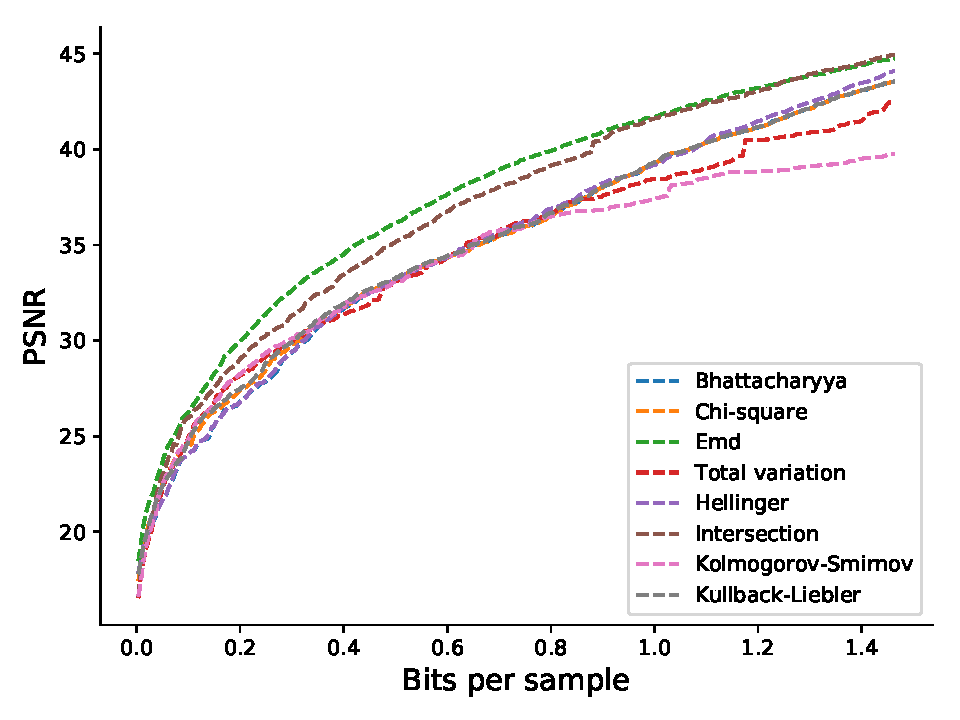
\includegraphics[width=0.48\linewidth]{img/histogram/different-metrics/turbulence-histogram-metrics.pdf}}
	\caption{PSNR comparison of eight histogram metrics on four data sets. The streams are truncated to better highlight differences.}
	\label{fig:histogram-metrics-comparison}
\end{figure}

Streams that are optimized for EMD perform the best in terms of function's PSNR, according to Figure
\ref{fig:histogram-fig:ahistogram-metrics-comparison}. It is unclear, however, that PSNR should be a
meaningful criteria for evaluating histogram distance metrics. We therefore compare the different
metrics further by plotting the reconstructed histograms for the \emph{diffusivity} data set at
$0.24$ bits per sample. The results are shown in Figure \ref{fig:histogram-metrics-comparison2}.
Based on the results from both of these experiments, we have decided to use EMD as the metric of
choice in this paper to measure histogram error. \ptb{I do not see a
  differences in the histograms}

\begin{figure}
	\centering
	\subcaptionbox{Bhattacharyya}
	{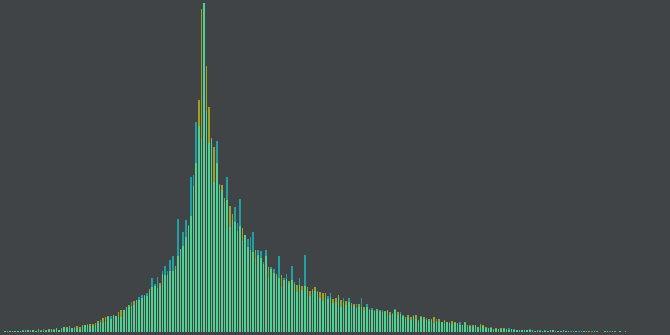
\includegraphics[width=0.24\linewidth]{img/histogram/different-metrics/bhattacharyya.png}}
	\subcaptionbox{Chi-square}
	{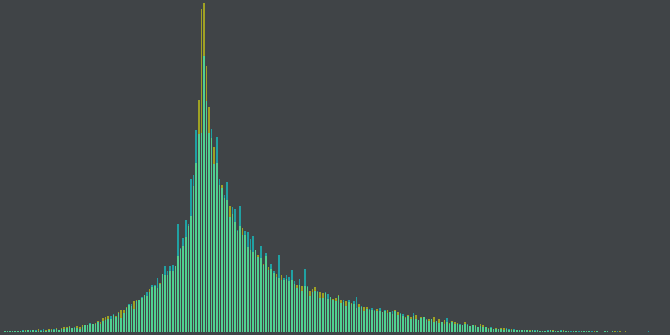
\includegraphics[width=0.24\linewidth]{img/histogram/different-metrics/chi_square.png}}
	\subcaptionbox{Emd}
	{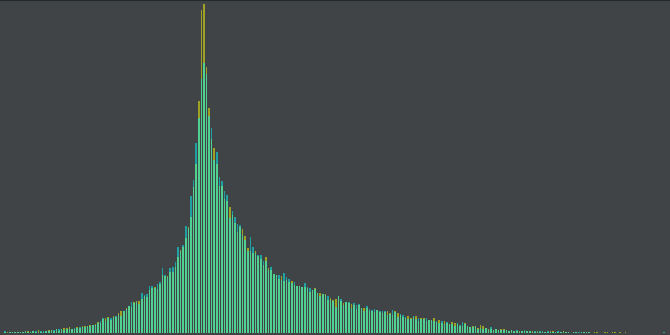
\includegraphics[width=0.24\linewidth]{img/histogram/different-metrics/emd.png}}
	\subcaptionbox{Hellinger}
	{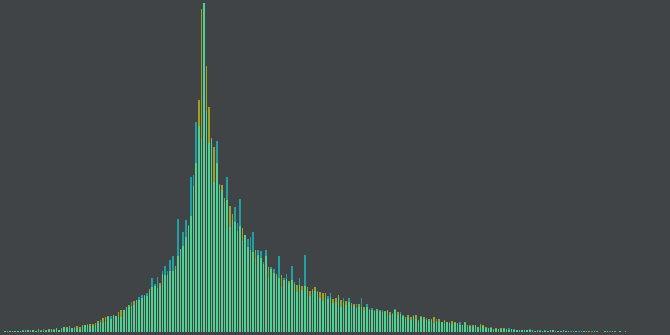
\includegraphics[width=0.24\linewidth]{img/histogram/different-metrics/hellinger.png}}
	\subcaptionbox{Total variation}
	{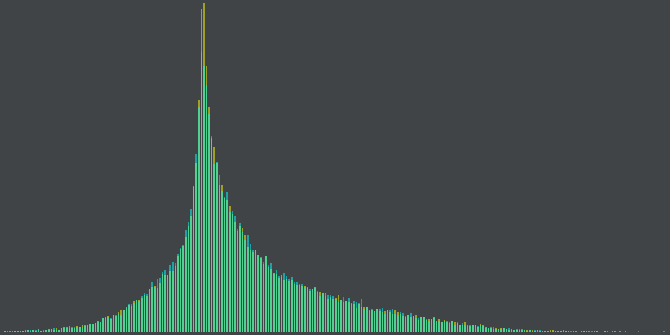
\includegraphics[width=0.24\linewidth]{img/histogram/different-metrics/total_variation.png}}
	\subcaptionbox{Intersection}
	{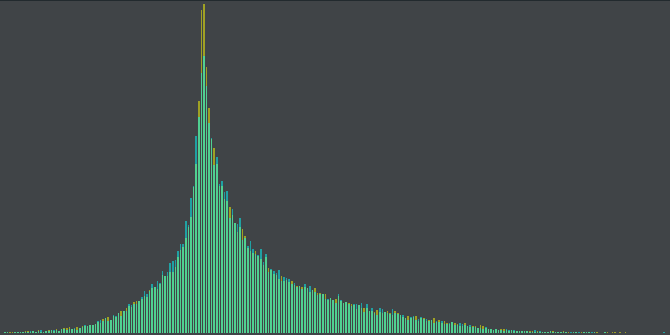
\includegraphics[width=0.24\linewidth]{img/histogram/different-metrics/intersection.png}}
	\subcaptionbox{Kolmogorov-Smirnov}
	{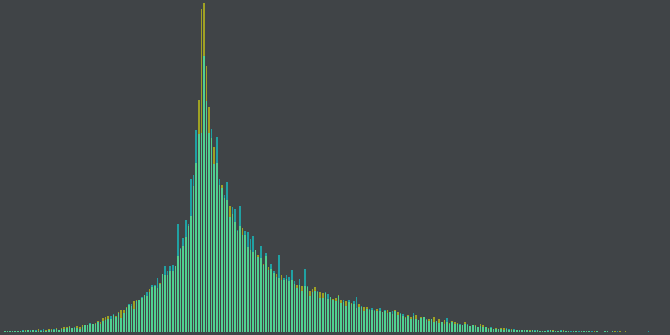
\includegraphics[width=0.24\linewidth]{img/histogram/different-metrics/kolmogorov_smirnov.png}}
	\subcaptionbox{Kullback-Liebler}
	{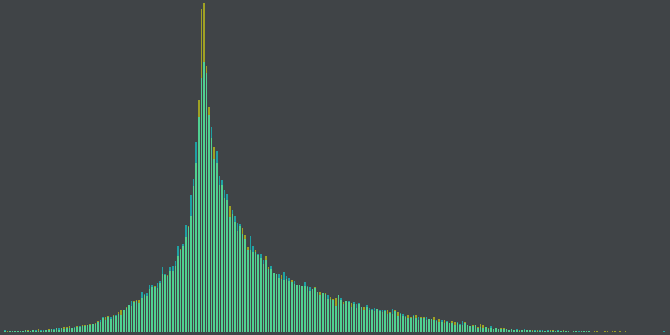
\includegraphics[width=0.24\linewidth]{img/histogram/different-metrics/kullback_liebler.png}}
	\caption{Reconstructed histograms for \emph{diffusivity} at $0.24$ bits per sample.}
	\label{fig:histogram-metrics-comparison2}
\end{figure}

With an error metric defined, Algorithm [REF] gives us a \emph{histogram-optimized} stream, given an
input data set. To understand the characteristics of an \emph{histogram-optimized} stream that make
it suitable for histogram computation, we compare it with the \emph{rmse-optimized} stream for the
same data set. Both of these streams, however, are data-dependent, and thus are impractical to
implement on the data receiving side as they require access to the whole data set to compute.
Therefore we also include the corresponding data-independent streams, namely \emph{histogram
signature} and \emph{by wavelet norm} (the concept of a signature is defined in Section [REF]).
Figures \ref{fig:histogram-stream-comparison} (a, c, e, g) are plots of the EMD errors for these
streams on four data sets. Figures \ref{fig:histogram-stream-comparison} (b, d, f, h) show the same
plots, except the leading zero bits are removed from each stream to mimic the effects of
compression often used in practice.

\begin{figure}
	\centering
	\subcaptionbox{\emph{boiler}}
	{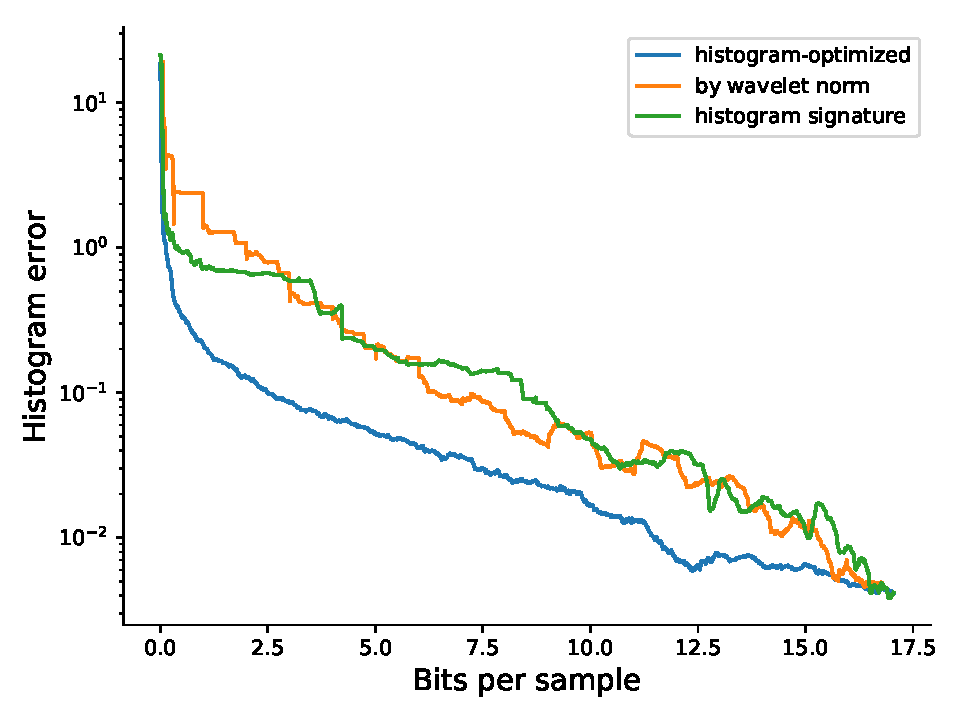
\includegraphics[width=0.48\linewidth]{img/histogram/boiler-histogram.pdf}}
	\subcaptionbox{\emph{boiler}, without leading zeros}
	{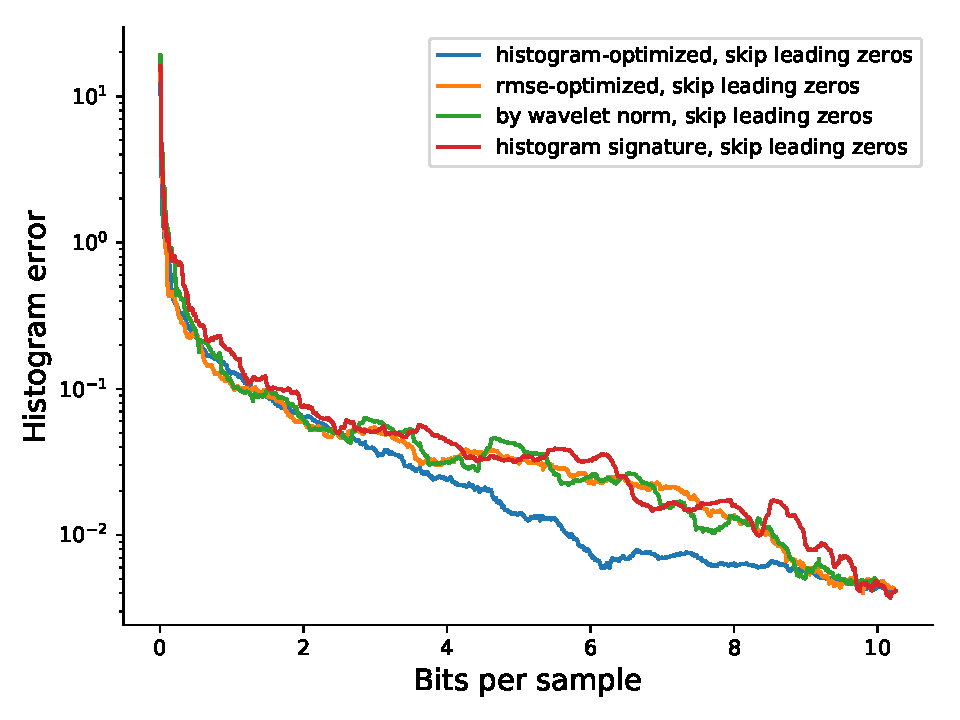
\includegraphics[width=0.48\linewidth]{img/histogram/skip-leading-zeros/boiler-histogram.pdf}}
	\subcaptionbox{\emph{flame}}
	{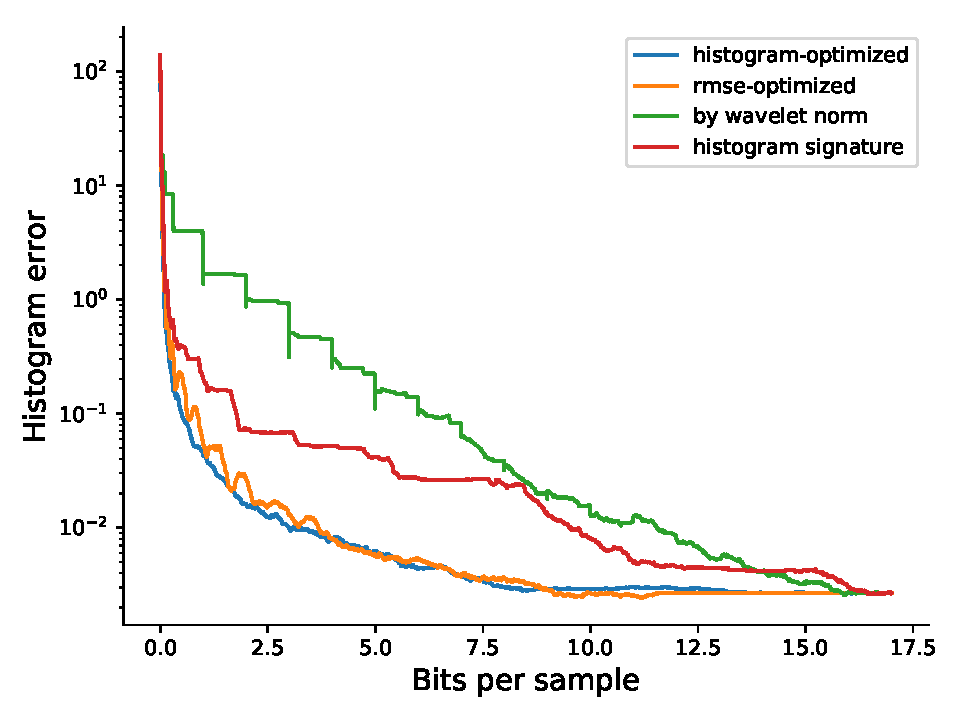
\includegraphics[width=0.48\linewidth]{img/histogram/kflame-histogram.pdf}}
	\subcaptionbox{\emph{flame}, without leading zeros}
	{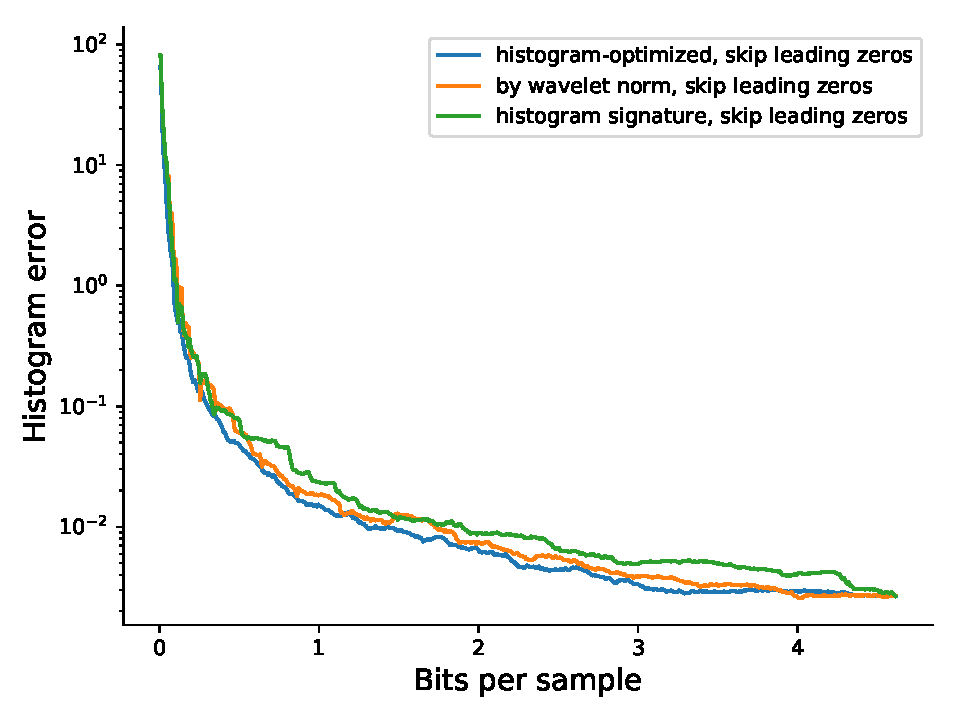
\includegraphics[width=0.48\linewidth]{img/histogram/skip-leading-zeros/kflame-histogram.pdf}}
	\subcaptionbox{\emph{diffusivity}}
	{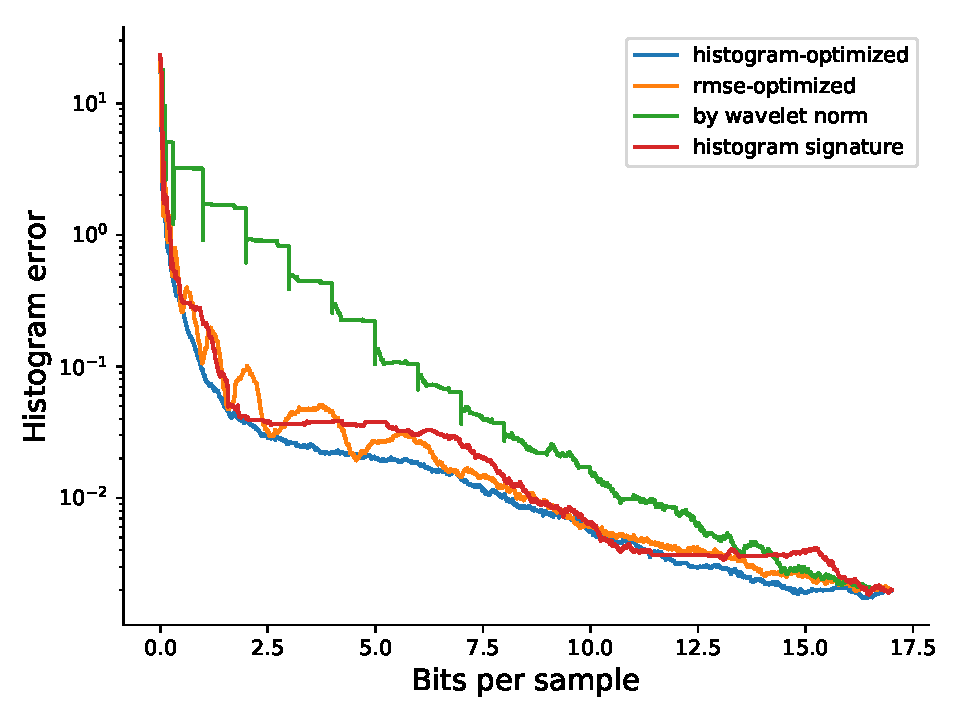
\includegraphics[width=0.48\linewidth]{img/histogram/miranda-diffusivity-histogram.pdf}}
	\subcaptionbox{\emph{diffusivity}, without leading zeros}
	{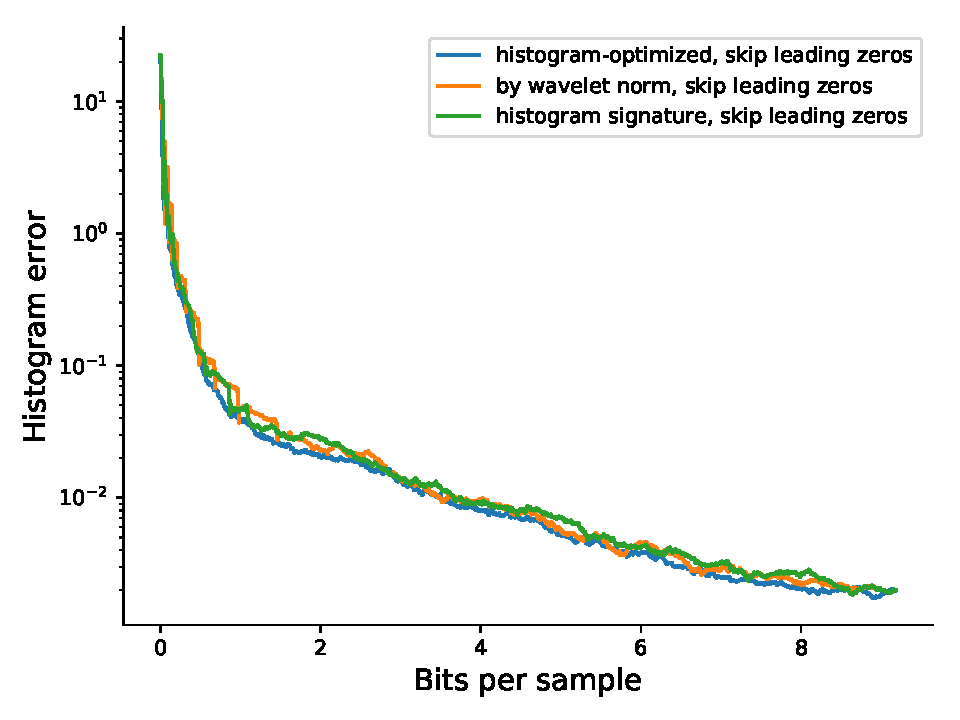
\includegraphics[width=0.48\linewidth]{img/histogram/skip-leading-zeros/miranda-diffusivity-histogram.pdf}}
	\subcaptionbox{\emph{turbulence}}
	{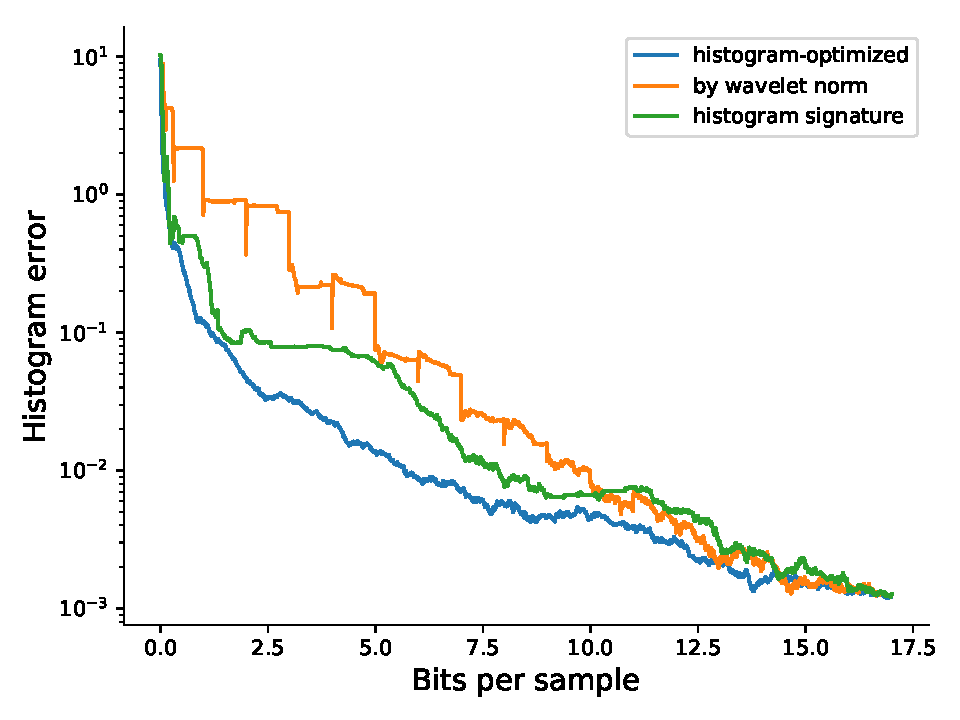
\includegraphics[width=0.48\linewidth]{img/histogram/turbulence-histogram.pdf}}
	\subcaptionbox{\emph{turbulence}, without leading zeros}
	{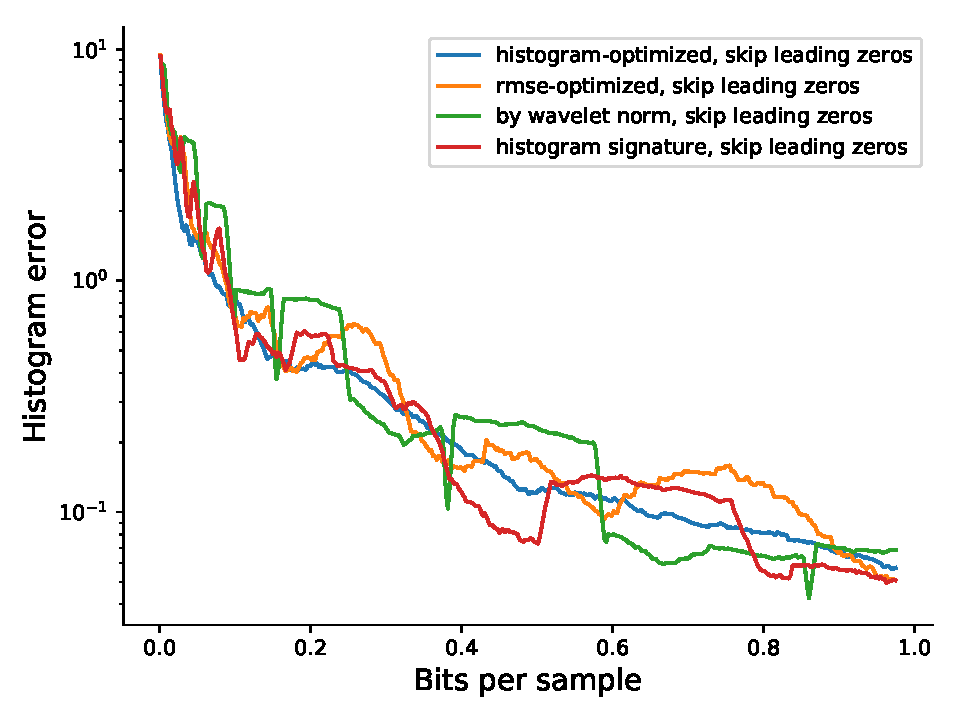
\includegraphics[width=0.48\linewidth]{img/histogram/skip-leading-zeros/turbulence-histogram.pdf}}
	\caption{EMD error comparison among four streams \emph{histogram-optimized},
	\emph{rmse-optimized}, \emph{by wavelet norm}, and \emph{histogram signature}, with (left) and
	without (right)	the leading zero bits. For the case of without leading zero bits (right), the
	plots are truncated to make the differences large enough for visual inspection, and trunction
	points are chosen so that the difference between the best of the reconstructed histograms and the
	groundtruth histogram is negligibly small.}
	\label{fig:histogram-stream-comparison}
\end{figure}

The are two observations to have from Figures \ref{fig:histogram-stream-comparison} (a, c, e, g).
First, compared to \emph{rmse-optimized}, the \emph{histogram-optimized} stream produces
consistently better histograms. Second, between the two data-independent streams, \emph{histogram
signature} outperforms \emph{by wavelet norm}. To better understand how the Earth mover's distance
translates to visual differences, we visualize the histograms produced by the different streams, at
low bit rates, in Figure \ref{fig:histogram-comparison-low-bit-rate}. These plots confirm our
observations.

\begin{figure}
	\centering
	\subcaptionbox{\emph{histogram-optimized}\\ emd = 0.42}
	{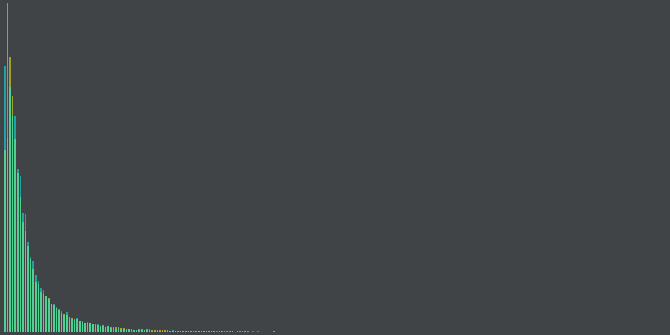
\includegraphics[width=0.24\linewidth]{img/histogram/turbulence-wlz/histogram.png}}
	\subcaptionbox{\emph{rmse-optimized}\\ emd = 0.77}
	{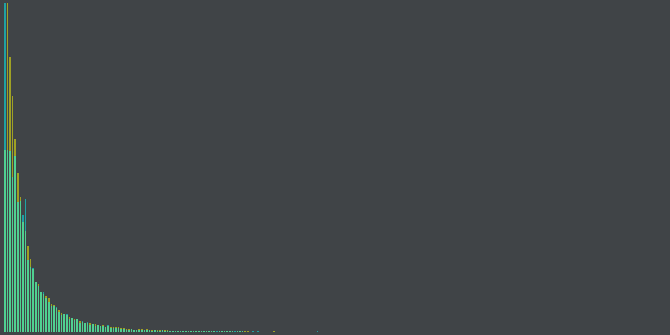
\includegraphics[width=0.24\linewidth]{img/histogram/turbulence-wlz/rmse.png}}
	\subcaptionbox{\emph{by wavelet norm}\\ emd = 4.24}
	{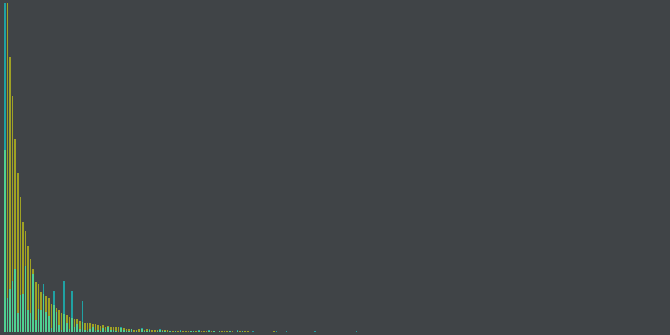
\includegraphics[width=0.24\linewidth]{img/histogram/turbulence-wlz/wavenorm.png}}
	\subcaptionbox{\emph{histogram signature}\\ emd = 0.54}
	{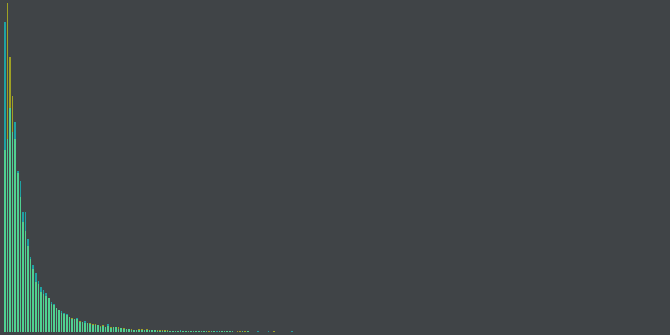
\includegraphics[width=0.24\linewidth]{img/histogram/turbulence-wlz/signature.png}}
	\subcaptionbox{\emph{histogram-optimized}\\ emd = 1.11}
	{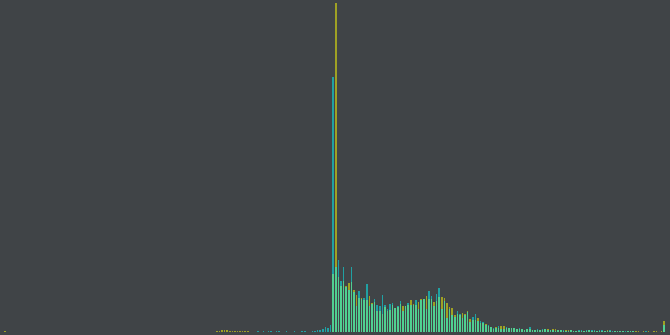
\includegraphics[width=0.24\linewidth]{img/histogram/boiler-wlz/histogram.png}}
	\subcaptionbox{\emph{rmse-optimized}\\ emd = 0.97}
	{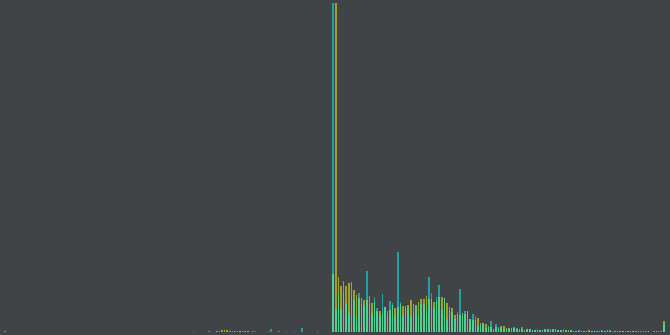
\includegraphics[width=0.24\linewidth]{img/histogram/boiler-wlz/rmse.png}}
	\subcaptionbox{\emph{by wavelet norm}\\ emd = 3.98}
	{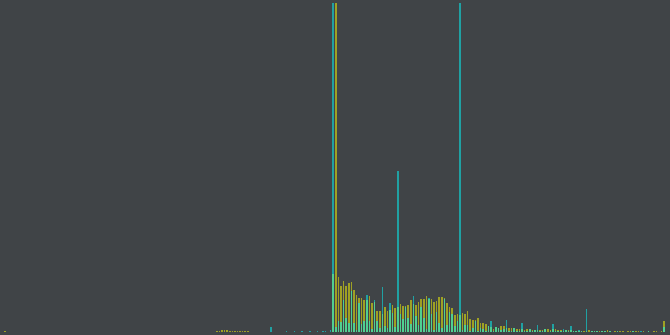
\includegraphics[width=0.24\linewidth]{img/histogram/boiler-wlz/wavenorm.png}}
	\subcaptionbox{\emph{histogram signature}\\ emd = 1.71}
	{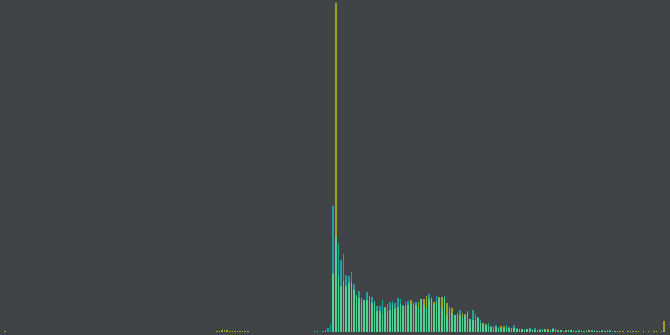
\includegraphics[width=0.24\linewidth]{img/histogram/boiler-wlz/signature.png}}
	\subcaptionbox{\emph{histogram-optimized}\\ emd = 0.40}
	{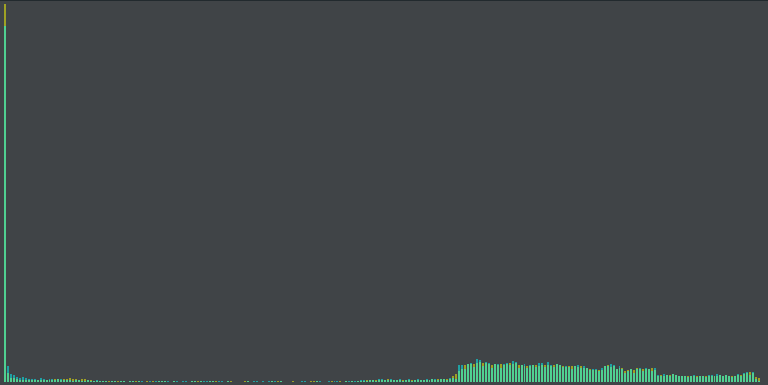
\includegraphics[width=0.24\linewidth]{img/histogram/kflame-wlz/histogram.png}}
	\subcaptionbox{\emph{rmse-optimized}\\ emd = 0.84}
	{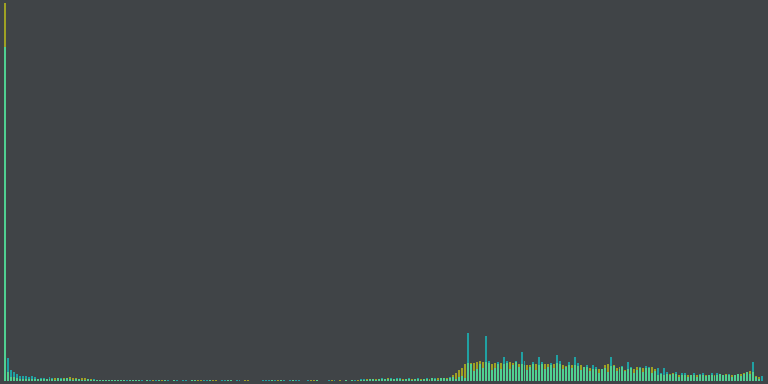
\includegraphics[width=0.24\linewidth]{img/histogram/kflame-wlz/rmse.png}}
	\subcaptionbox{\emph{by wavelet norm}\\ emd = 8.49}
	{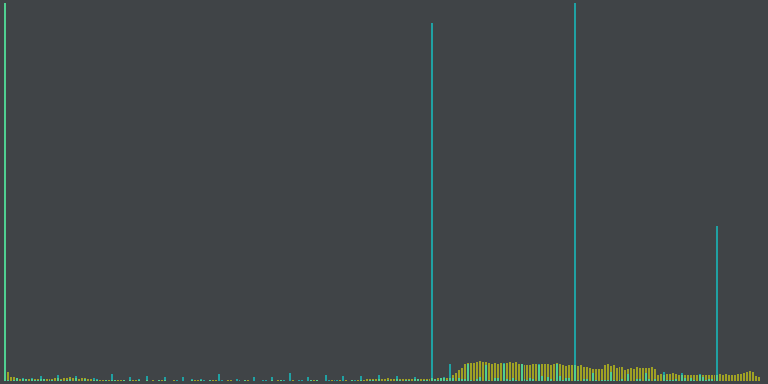
\includegraphics[width=0.24\linewidth]{img/histogram/kflame-wlz/wavenorm.png}}
	\subcaptionbox{\emph{histogram signature}\\ emd = 1.03}
	{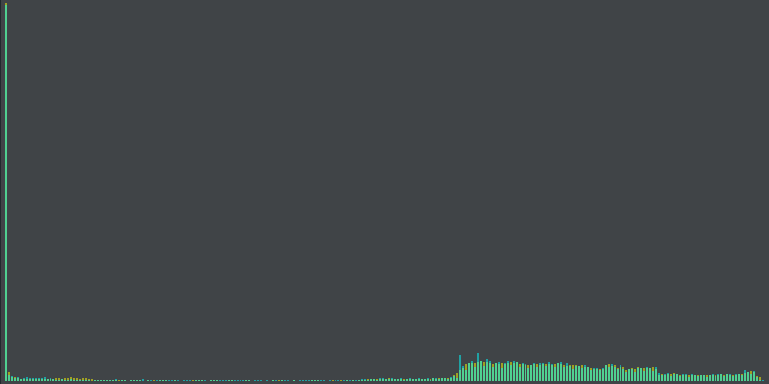
\includegraphics[width=0.24\linewidth]{img/histogram/kflame-wlz/signature.png}}
	\subcaptionbox{\emph{histogram-optimized}\\ emd = 0.58}
	{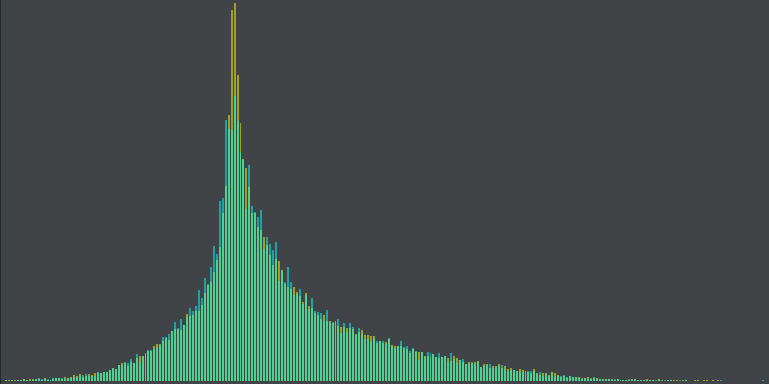
\includegraphics[width=0.24\linewidth]{img/histogram/diffusivity-wlz/histogram.png}}
	\subcaptionbox{\emph{rmse-optimized}\\ emd = 1.14}
	{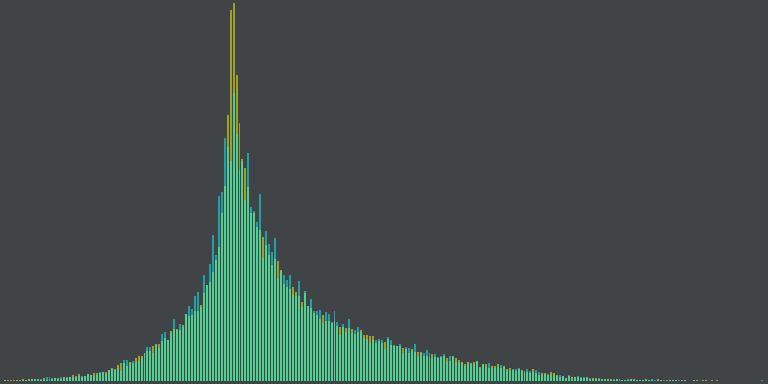
\includegraphics[width=0.24\linewidth]{img/histogram/diffusivity-wlz/rmse.png}}
	\subcaptionbox{\emph{by wavelet norm}\\ emd = 5.07}
	{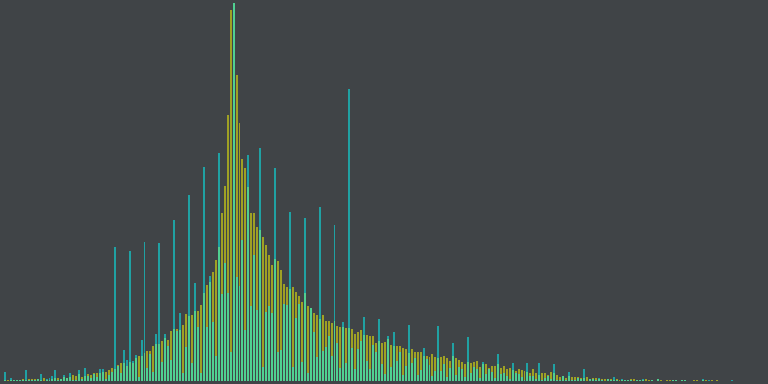
\includegraphics[width=0.24\linewidth]{img/histogram/diffusivity-wlz/wavenorm.png}}
	\subcaptionbox{\emph{histogram signature}\\ emd = 3.87}
	{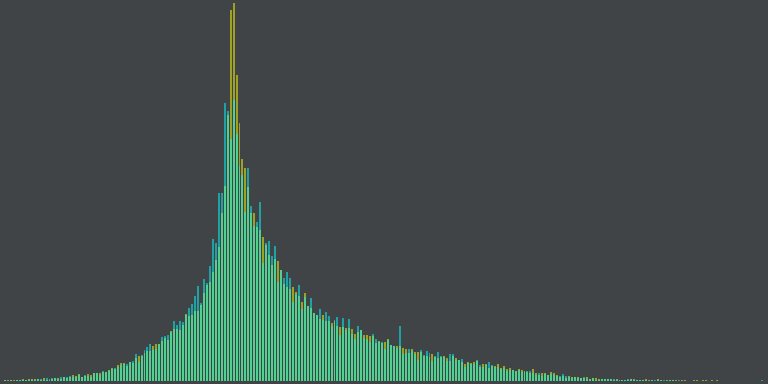
\includegraphics[width=0.24\linewidth]{img/histogram/diffusivity-wlz/signature.png}}
	\caption{Histograms at low bit rates. (a,b,c,d) turbulence at 0.3 bps, (e,f,g,h) boiler at 0.1
	bps, (i,j,k,l) flame at 0.2 bps, (m,n,o,p) diffusivity at 0.3 bps.}
	\label{fig:histogram-comparison-low-bit-rate}
\end{figure}

The main difference between the \emph{histogram-optimized} and the \emph{rmse-optimized} streams is
that \emph{histogram-optimized} favors low-ordered bits of coarse-level coefficients, while,
\emph{rmse-optimized} relatively favors high-ordered bits of fine-level coefficients. This is
evident in Figure \ref{fig:histogram-signature-comparison} (b and d): for
\emph{histogram-optimized}, the bright blue cells extend more toward the right (lower-ordered bit
planes) and less toward the bottom (finer resolution levels). The histogram experiments in this
Section are performed with 256 bins, but this fact holds for a wide range of number of bins. Figures
\ref{fig:histogram-signature-comparison} (a, b, c) show that varying the number of bins from 128 to
512 only affects the relative ordering among the low-ordered bits on very fine resolution levels
(the dark blue cells at the bottom right of the signature). These are bits that come at the end of a
stream, and thus matter little to the data quality. 
 
\begin{figure}
	\centering
	\subcaptionbox{\emph{histogram-optimized}'s signature,\\ 128 bins}
	{
\includegraphics[width=0.24\linewidth]{img/histogram/sig-GREEDY-(histogram-128).png}}
	\subcaptionbox{\emph{histogram-optimized}'s signature,\\ 256 bins}
	{
\includegraphics[width=0.24\linewidth]{img/histogram/sig-GREEDY-(histogram-256).png}}
	\subcaptionbox{\emph{histogram-optimized}'s signature,\\ 512 bins}
	{
\includegraphics[width=0.24\linewidth]{img/histogram/sig-GREEDY-(histogram-512).png}}
	\subcaptionbox{\emph{rmse-optimized}'s signature}
	{
\includegraphics[width=0.24\linewidth]{img/histogram/sig-GREEDY-(rmse).png}}
	\caption{\emph{histogram-optimized}'s signature and \emph{rmse-optimized}'s signature}
	\label{fig:histogram-signature-comparison}
\end{figure}

When leading zero bits are removed from streams, all four streams become closer in EMD error (Figure
\ref{fig:histogram-stream-comparison} (b, d, f, h)). This is because, if the leading zero bits are
present, they serve as a `'cost'' that streams must pay to approach the (later) significant bits.
All streams have to pay that cost, but streams that favor resolution over precision pay more in the
beginning, because in practice, most of the leading zero bits concentrate in fine-resolution levels.
Therefore the removal of leading zero bits impacts a resolution-favoring stream, e.g.,
\emph{rmse-optimized}, more than it impacts a precision-favoring stream such as
\emph{histogram-optimized}. Even though the streams become closer in EMD, their relative performance
largely stays the same, that is, \emph{histogram-optimized} and \emph{histogram signature}
outperform \emph{rmse-optimized} and \emph{by wavelet norm} respectively. For example, Figure
\ref{fig:histogram-comparison-low-bit-rate-slz} shows the four reconstructed histograms at 0.1 bits
per sample, with leading zero bits removed, for the diffusivity data set.

\begin{figure}
	\centering
	\subcaptionbox{\emph{histogram-optimized},\\ without leading zeros}
	{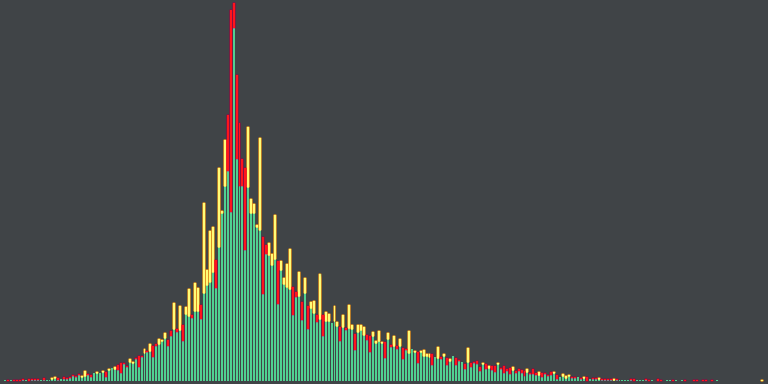
\includegraphics[width=0.24\linewidth]{img/histogram/diffusivity/histogram.png}}
	\subcaptionbox{\emph{rmse-optimized},\\ without leading zeros}
	{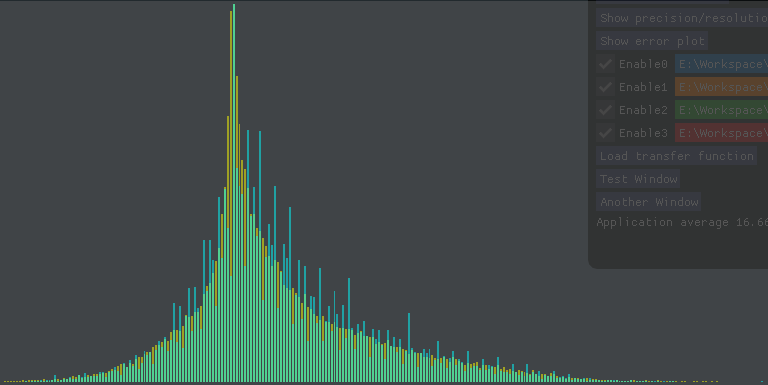
\includegraphics[width=0.24\linewidth]{img/histogram/diffusivity/rmse.png}}
	\subcaptionbox{\emph{by wavelet norm},\\ without leading zeros}
	{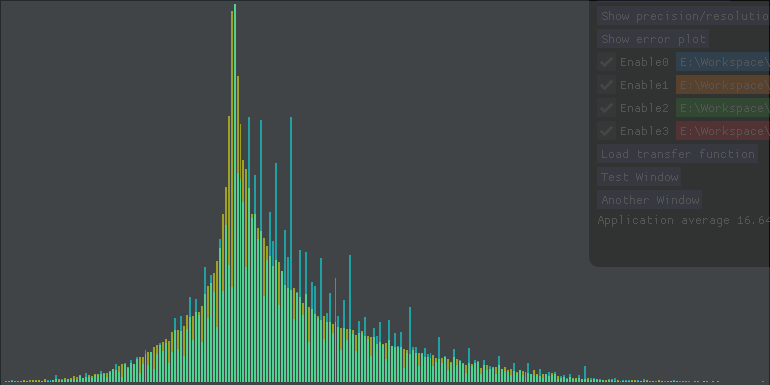
\includegraphics[width=0.24\linewidth]{img/histogram/diffusivity/wavenorm.png}}
	\subcaptionbox{\emph{histogram signature},\\ without leading zeros}
	{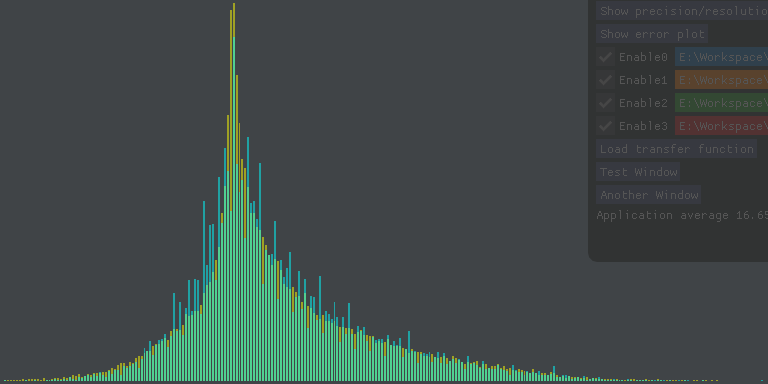
\includegraphics[width=0.24\linewidth]{img/histogram/diffusivity/signature.png}}
	\caption{diffusivity's histograms at 0.1 bps, without leading zero bits. }
	\label{fig:histogram-comparison-low-bit-rate-slz}
\end{figure}

The streams in Figure \ref{fig:histogram-comparison-low-bit-rate} (b, d, f, h) are truncated where
the EMD errors of the \emph{histogram-optimized} streams are negligible, suggesting that it is often
possible to achieve near lossless histograms with just 1 bit per sample. The boiler data set is a
peculiar case, where the \emph{histogram-optimized} stream outperforms the rest of the streams by a
large margin in the second half of the bit rate range. Looking at the precision maps (defined in
Section [REF]) for the \emph{histogram-optimized} stream, as well as its reconstructed histogram
(Figure \ref{fig:precision-map-histogram}, (a)), we see that the bit distribution is heavily
concentrated in regions corresponding to one particular histogram bin that contains vastly more
samples than other bins do. This situtation happens when there are many samples having essentially
the same value but they are distributed irregularly in space (otherwise they would form constant
regions which would be captured very well with just a few precision bits of wavelet coefficients --
this is the case for the flame data set). In this case a stream needs to be more spatially adaptive
to resolve well the histogram bin with the most samples, and among the tested streams, only
\emph{histogram-optimized} is spatially adaptive to EMD (\emph{rmse-optimized} is spatially
adaptive, but to RMSE, and the other two streams are data-independent).

\begin{figure}
	\centering
	\subcaptionbox{}
	{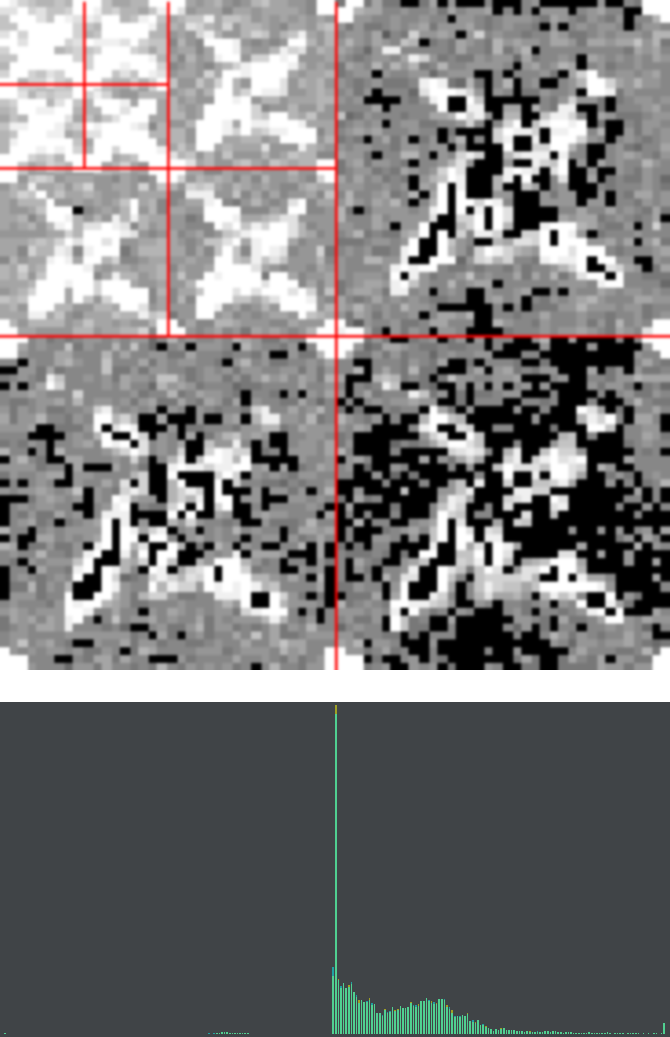
\includegraphics[width=0.24\linewidth]{img/histogram/boiler/prec-histogram_resize-vert.png}}
	\subcaptionbox{}
	{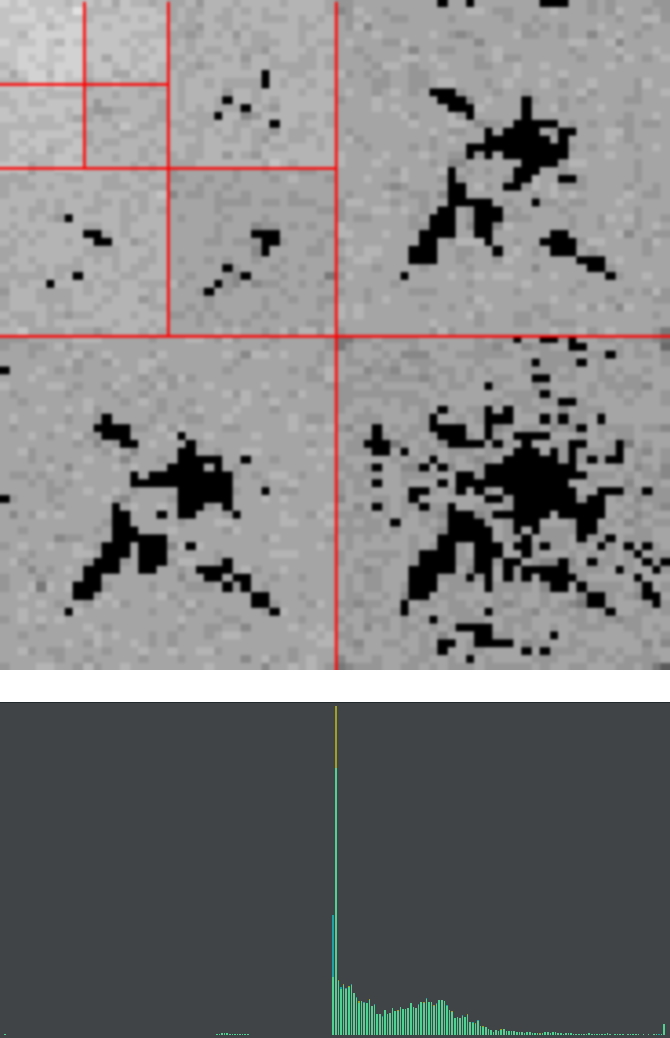
\includegraphics[width=0.24\linewidth]{img/histogram/boiler/prec-rmse_resize-vert.png}}
	\subcaptionbox{}
	{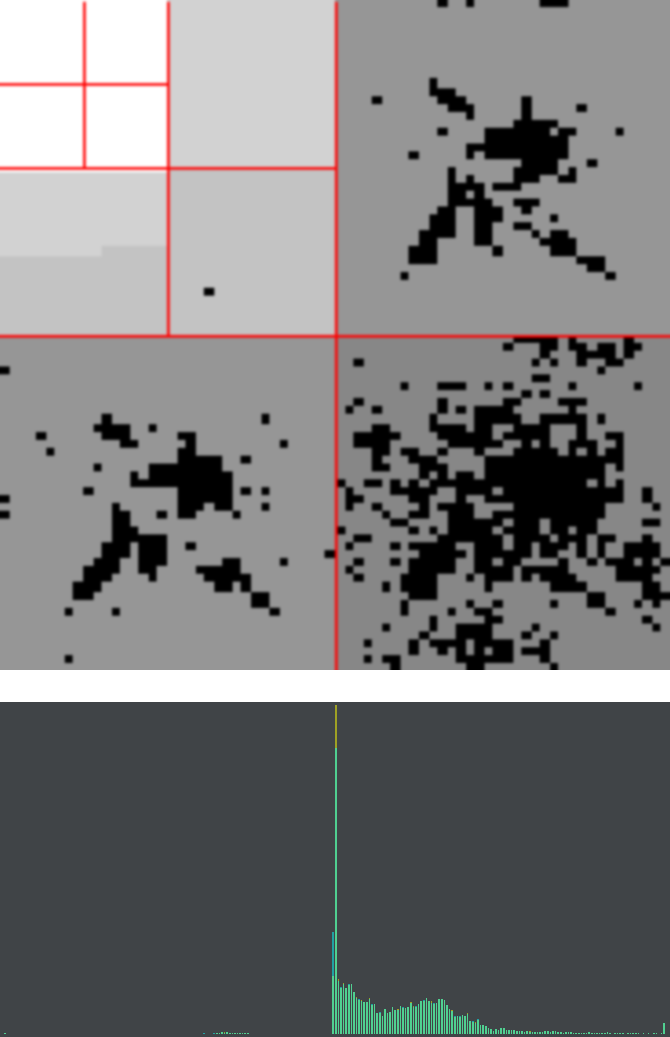
\includegraphics[width=0.24\linewidth]{img/histogram/boiler/prec-signature_resize-vert.png}}
	\subcaptionbox{}
	{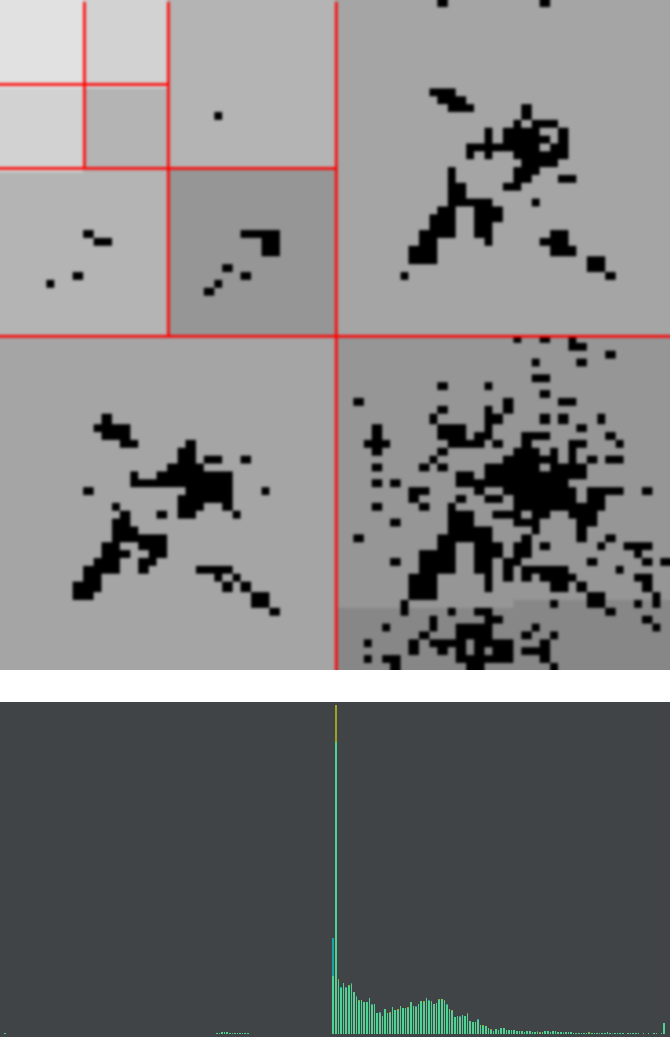
\includegraphics[width=0.24\linewidth]{img/histogram/boiler/prec-wavenorm_resize-vert.png}}
	\caption{(top) Precision distribution of wavelet coefficients, and (bottom) reconstructed
	histograms, for \emph{histogram-optimized}, \emph{rmse-optimized}, \emph{by wavelet norm}, and
	\emph{histogram signature} streams, at 6.47 bits per sample, without leading zero bits.}
	\label{fig:precision-map-histogram}
\end{figure}

In this section we have shown that histogram computation requires a different ordering of bits than
reconstructing the function itself. We have also proposed a practical heuristic, based on stream
signatures, to capture the main characteristics of this ordering. In practice, the histogram
signature can be pre-computed once and stored on disk. A signature's size is negligible (170
integers in 2D and 374 integers in 3D in the case of four wavelet levels in each dimension), and can
also be further compressed. Therefore it can be transmitted first, and the receiver of the data can
ultilize the signature to smartly query the bits so as to reconstruct the data's histogram with as
few bits as possible.
%%% Local Variables:
%%% mode: latex
%%% TeX-master: "template"
%%% End:
